\section{The Quasi-Geostrophic potential
vorticity}\label{the-quasi-geostrophic-potential-vorticity}

\subsection{The equations of motion}\label{the-equations-of-motion}

The quasi geostrophic approximation is a low Rossby number, high
Richardson number approximation to the hydrostatic primitive equations.
The hydrostatic primitive equations have been used in most global
circulation models for many years, but they incorporate a number of
approximations that are becoming increasingly inadequate as the
resolution of the models increases and the accuracy of the processes
included raise the standard of detail required.

Some approximations are rather solid, like the assumptions of sphericity
of the Earth gravitational potential, whose deviations are measurable,
but probably minor for atmospheric motions, and the neglect of Coriolis
terms including the cosine of latitude, even if the latter has been
subject to a lot of discussions. The third major simplification is the
hydrostatic approximation that is required to eliminate from the
equation acoustic waves, generated by density variations, that
complicate their numerical solution and are rather ineffectual for
atmospheric motions. However, removing all density differences would be
too strict for the atmosphere, so another approximation is required that
though eliminating the sound waves is capable of retaining the
compressible character of the fluid. Such an approximation was found by
Boussinesq (Joseph Velentin Boussinesq, 1842-1929).White2005 provides a
nice review of the approximations.

The Boussinesq approximation stems from the necessity of eliminating
fast compressible waves (sound waves or elastic waves) when this kind of
motions are not relevant. As we have discussed, the most drastic way is
require the flow to have constant density

\[\rho = const.\]

but this hypothesis is a very poor approximation. The Boussinesq
approximation will retain some of the density variations when they are
coupled to gravity that is sufficiently strong to give to the product
the magnitude to be important for the atmpsheric motions. In this way
the Boussinesq approximation belongs to the class of anelastic
approximations, first proposed by Ogura1962.

\subsection{The Boussinesq equation for the
atmosphere}\label{the-boussinesq-equation-for-the-atmosphere}

The motions are therefore small variations with respect a much larger
reference state. This means that the atmosphere is almost always in an
approximate, but strongly maintained balance both vertically and
horizontally. We can therefore introduce a separations in the density
and the pressure

\[\begin{aligned}
\rho(x,y,z,t) &= \rho_0+ \rho'(x,y,z,t)+\tilde{\rho}(z)   \\
p(x,y,z,t) &=  p'(x,y,z,t)+\tilde{p}(z)
\end{aligned}\]

where \(\rho_0\) is a constant density characteristic of the flow and
the reference state is in hydrostatic balance

\[\frac{\partial \tilde{p}}{\partial z} = -g \tilde{\rho}\]

The equations of motion then are

{\[\begin{aligned}
&\frac{\partial u}{\partial t} = -u\frac{\partial u}{\partial x} -v\frac{\partial u}{\partial y} -w\frac{\partial u}{\partial z} +  f v -\frac{1}{\rho}\frac{\partial p}{\partial x}  \\ 
&\frac{\partial v}{\partial t} = -u\frac{\partial v}{\partial x} -v\frac{\partial v}{\partial y} -w\frac{\partial v}{\partial z} -  f u -\frac{1}{\rho}\frac{\partial p}{\partial y}  \\
&\frac{\partial w}{\partial t} = -u\frac{\partial w}{\partial x} -v\frac{\partial w}{\partial y} -w\frac{\partial w}{\partial z} -\frac{1}{\rho}\frac{\partial p}{\partial z} -g\\
&\frac{\partial \rho}{\partial t} + \left(\frac{\partial (u\rho)}{\partial x} +\frac{\partial (v\rho)}{\partial y} +\frac{\partial (w\rho)}{\partial z}\right) = 0
\end{aligned}\]}

we will now introduce the incompressibility condition

\[\frac{D \rho}{Dt} = 0\]

than the continuity equation reduces to \(\nabla\cdot\mathbf{v}= 0\).
Introducing the separation of the reference state and neglecting the
variation of density with respect the constant density,

\[\frac{\rho-\rho_0}{\rho_0} \ll 1\]

unless it is coupled to buoyancy, we get the Boussinesq approximated set
for adiabatic inviscid flow

\[\begin{aligned}
&\frac{D u}{Dt} =    f v -\frac{1}{\rho_0}\frac{\partial p}{\partial x}  \\ 
&\frac{D v}{Dt} =  -  f u -\frac{1}{\rho_0}\frac{\partial p}{\partial y} \label{eq:PE1} \\
&\frac{D w}{Dt} =  b \\
&\frac{D b}{Dt} + N^2 w = 0 \\
&\frac{\partial  u}{\partial x}+\frac{\partial  v}{\partial y}+\frac{\partial w}{\partial z} =0
\end{aligned}\]

where \(f=f_0 +\beta y\), and we have defined the buoyancy \(b\) as
\(b=g\rho'/\rho_0\). The stratification of the reference state is
indicated by

\[N^2 = -\frac{g}{\rho_0}\frac{d \tilde{\rho}}{dz}\]

If the fluid is a liquid these equations are quite appropriate and they
are consistent, but if the fluid is a compressible gas we need a little
bit more work. In this case we will find similar definitions for
\(\tilde{p}, b , N^2\), but they will be defined in terms of potential
temperature \(\theta\) and \(\pi =(\frac{p}{p_s})^{R/c_p}\), so that
\(T=\theta \pi\). Then

\[\frac{1}{\rho}\nabla p = c_p \theta \nabla\pi\]

and the hydrostatic balance for the reference state can then be written
as

\[c_p\tilde{\theta}\frac{d \tilde{\pi}}{dz} = -g\]

The momentum equations (\texttt{eq:PE0}) can then be expressed in the
new variables

{\[\begin{aligned}
&\frac{D u}{Dt} =  +  f v +c_p\theta\frac{\partial \pi}{\partial x}  \\ 
&\frac{D v}{Dt} =  -  f u +c_p\theta\frac{\partial \pi}{\partial y}  \\
&\frac{D w}{Dt} =  c_p\theta\frac{\partial \pi}{\partial z} -g\\
\end{aligned}\]}

introducing the reference state and subtracting the hydrostatic balance
for the reference state

{\[\begin{aligned}
&\frac{D u}{Dt} =  +  f v -c_p\theta\frac{\partial \pi'}{\partial x}  \\ 
&\frac{D v}{Dt} =  -  f u -c_p\theta\frac{\partial \pi'}{\partial y}  \\
&\frac{D w}{Dt} =  -c_p\theta\frac{\partial \pi'}{\partial z} -g\frac{\theta'}{\tilde{\theta}}\\
\end{aligned}\]}

The Boussinesq approximation can now be used also here, but in terms of
the new variables it is expressed as neglecting the variation of the
potential temperature except in the leading order contribution to the
buoyancy. This can be achieved by introducing the new quantities

\[\begin{aligned}
p' &= c_p\theta\pi' \\
b' &= g\frac{\theta'}{\theta_0} \\
N^2&= \frac{g}{\theta_0}\frac{d \tilde{\theta}}{dz}
\end{aligned}\]

the Boussinesq equation for a compressible fluid will then be formally
identical to the Boussinesq equation for an incompressible fluid :

{\[\begin{aligned}
&\frac{\partial u}{\partial t} = -u\frac{\partial u}{\partial x} -v\frac{\partial u}{\partial y} -w\frac{\partial u}{\partial z} +  f v -\frac{\partial p'}{\partial x}  \\ 
&\frac{\partial v}{\partial t} = -u\frac{\partial v}{\partial x} -v\frac{\partial v}{\partial y} -w\frac{\partial v}{\partial z} -  f u -\frac{\partial p'}{\partial y}  \\
&\frac{\partial p'}{\partial z} = g\frac{\theta'}{\theta_0} \\
&\frac{\partial b'}{\partial t} = -u\frac{\partial b'}{\partial x} -v\frac{\partial b'}{\partial y} -w\frac{\partial b'}{\partial z}  - N^2  w \\
&\frac{\partial u}{\partial x}+\frac{\partial v}{\partial y}+\frac{\partial w}{\partial z}=0
\end{aligned}\]}

Incorporating constants into the definitions and dropping primes we can
write the equations more simply as

{\[\begin{aligned}
&\frac{\partial u}{\partial t} = -u\frac{\partial u}{\partial x} -v\frac{\partial u}{\partial y} -w\frac{\partial u}{\partial z} +  f v -\frac{\partial p'}{\partial x}  \\ 
&\frac{\partial v}{\partial t} = -u\frac{\partial v}{\partial x} -v\frac{\partial v}{\partial y} -w\frac{\partial v}{\partial z} -  f u -\frac{\partial p'}{\partial y}  \\
&\frac{\partial p}{\partial z} = \theta \\
&\frac{\partial b}{\partial t} = -u\frac{\partial b}{\partial x} -v\frac{\partial b}{\partial y} -w\frac{\partial b}{\partial z}  - N^2  w \\
&\frac{\partial u}{\partial x}+\frac{\partial v}{\partial y}+\frac{\partial w}{\partial z}=0
\end{aligned}\]}

The mean static stability is defined by
\(N^2 = \frac{g}{\theta_0}\frac{d \tilde{\theta}}{dz}=\frac{\partial \tilde{b}}{\partial z}\)

\subsection{Scales of motion}\label{scales-of-motion}

We introduce scales for the basic variables

{\[(x,y) \approx L, \quad (u,v) \approx U, \quad t\approx \frac{U}{L},\quad z\approx H, \quad f\approx f_0\]}

We will define adimensional quantity from the horizontal velocity scale,
\(U\) and the horizontal space scale \(L\) as (Rossby number)

\[\text{Ro} = \frac{U}{f_0 L} \approx \frac{\zeta}{f}\]

a small value of \(Ro\) implies a small relative vorticity with respect
the planetary vorticity, indicating that the rotation effects are
dominant. In this case the dominant balance is between the Coriolis
terms and the pressure gradient term. This will give us the scaling of
the pressure

\[f U \approx P/L\]

so \(P \approx f_0 U L\). The hydrostatic relation produces the scale
for the buoyancy

{\[b'\approx B = P/H=f_0UL/H\]}

where the length \(L_d = \frac{HN}{f_0}\) is the deformation radius in
the stratified fluid.

We can then define another important adimensional number that is linked
to stratification and is called the Richardson number

\[\text{Ri} = \frac{N^2}{(\frac{\partial u}{\partial z})^2}\]

where \(N^2 =\frac{\partial b}{\partial z}\). Then the following
relations hold:

\[\begin{aligned}
\text{Ri} &= \frac{N^2H^2}{U^2} \\
\text{Ro}^2\text{Ri} &=\frac{N^2 H^2}{L^2 f^2}
\end{aligned}\]

The vertical velocity is adimensionalized using the mass conservation
equation

\[\left(\frac{\partial  u}{\partial x}+\frac{\partial  v}{\partial y}\right)=-\frac{\partial w}{\partial z}\]

suggesting that

\[W \approx \frac{U H}{L}.\]

For time scales of the motion close to the advective time scale \(L/U\)
we find that the advective acceleration is

\[\begin{aligned}
\frac{D u}{Dt} \approx Ro (f v)\\
\frac{D v}{Dt} \approx Ro (- f u)
\end{aligned}\]

indicating that the advection terms or smaller of order \(Ro\) than the
Coriolis terms. For small Rossby number then an approximate balance
exist between the Coriolis terms and the pressure gradient force

\[\begin{aligned}
v \approx v_g =  \frac{1}{f_0}\frac{\partial \tilde{p}}{\partial x}\\
u \approx u_g = -\frac{1}{f_0}\frac{\partial \tilde{p}}{\partial y}
\end{aligned}\]

(for motion of small meridional scale). From these relations we can
obtain a thermal wind relation

\[\begin{aligned}
\frac{\partial v_g}{\partial z} =  \frac{1}{f_0}\frac{\partial b}{\partial x}\\
\frac{\partial u_g}{\partial z} = -\frac{1}{f_0}\frac{\partial b}{\partial y}
\end{aligned}\]

and so we can deduce the horizontal scale of the variations of the
buoyancy \(b\)

\[\Delta b \approx \frac{f_0 L U}{H}\]

or

\[\frac{\Delta b}{H} \approx \frac{f_0 L U}{H^2}= \frac{f^2L^2}{H^2} Ro\]

and finally

\[\frac{\Delta b}{N^2 H} \approx \frac{f_0^2L^2}{N^2H^2} Ro = \frac{1}{Ro Ri}\]

A consistent requirement is that the Richardson number is larger than
1 so that

{\[Ro Ri \gg 1\]}

and

\[\frac{\Delta b}{H} \ll \frac{\partial b}{\partial z}\]

meaning that the variation of the static stability are smaller than the
static stability itself.

The combination of Rossby and Richardson numbers can also be written as

\[\frac{1}{Ro Ri} = Ro \frac{f_0^2L^2}{H^2N^2} = Ro\frac{L^2}{L_d^2}\]

where the length \(L_d = \frac{HN}{f_0}\) is the Rossby deformation
radius of the fluid. This relations show that the condition
(\texttt{cond1}) is equivalent to require

\[Ro\frac{L^2}{L_d^2} \ll 1\]

and so the for motion larger than the deformation radius \(L_d\) the
Rossby number must be small.

It is interesting to note here that the Richarson number can be
expressed as a ratio of lengths. This means that the vertical structure,
as expressed by the stratification of the reference state \(N^2\)
induces an horizontal scale. Another way of expressing th elink between
horizontal and vertical motions.

\subsection{The Rossby number
expansion}\label{the-rossby-number-expansion}

It is now possible to expand all variables as an asymptotic series of
the Rossby number

\[\mathbf{V}= \mathbf{V}_0 + Ro\,\mathbf{V}_1 + \cdots; \quad p=p_0 + Ro \, p_1 + \cdots ; \cdots\]

where we are now using two-dimensional vectors, \(\mathbf{V}= (u,v)\),
and horizontal advective derivative and gradients. The planetary
vorticity then can be expanded as \(f = f_0 + \beta y Ro/f_0\)

The expansion of the vertical velocity requires more care

\[\frac{D }{Dt} = \frac{\partial }{\partial t} + \mathbf{V}\cdot\nabla = \frac{\partial }{\partial t} + u\frac{\partial }{\partial x} + v\frac{\partial }{\partial y}.\]

At the zero order the momentum equations becomes

{\[v = \frac{1}{f_0}\frac{\partial p_0}{\partial x} \qquad u = -\frac{1}{f_0}\frac{\partial p_0}{\partial y}\]}

that implies that the zero order flow is horizontally non-divergent

\[\nabla \cdot\mathbf{V}_0 =0\]

as a consequence the mass conservation equation reduces to

\[\frac{\partial  w_0}{\partial z}=0\]

This relation shows that \(w\) is even smaller than our estimate scaling
\(UH/L\) might suggest. If there is a point where \(w_0\) is zero, then
it must zero everywhere. It could be nonzero on a bordering surface, but
in that case a vertical velocity of the order

\[w* \approx O(U \delta/L)\]

where \(\delta\) is the displacement of the surface and in adimensional
unit then

\[w \approx O(\delta/H)\]

so if we are limiting ourselves to the cases when \(O(\delta/H) = Ro\),
the first order vertical velocity is zero and then \(w = Ro\, w_1\).

The equations at the first order (Rossby number order) can then be
written as

{\[\begin{aligned}
\frac{\partial u_0}{\partial t}  + u_0\frac{\partial u_0}{\partial x} +v_0\frac{\partial u_0}{\partial y} -\beta y v_0 -  f_0 v_1 &= -\frac{\partial p_1}{\partial x}  \\ 
\frac{\partial v_0}{\partial t} +u_0\frac{\partial v_0}{\partial x} + v_0\frac{\partial v_0}{\partial y}  +\beta y u_0+  f_0 u_1  &= -\frac{\partial p_1}{\partial y}  \\
\frac{\partial \theta_0}{\partial t}  +u_0\frac{\partial \theta_0}{\partial x} +v_0\frac{\partial \theta_0}{\partial y}  + N^2(z) w_1   &= 0\\
\frac{\partial u_1}{\partial x}+\frac{\partial  v_1}{\partial y}+\frac{\partial w_1}{\partial z} &=0
\end{aligned}\]}

\subsection{The quasi-geostrophic potential vorticity
equation}\label{the-quasi-geostrophic-potential-vorticity-equation}

To obtain a single equation we cross differentiate the momentum
equations to obtain

{\[\frac{\partial \zeta_0}{\partial t} +(\mathbf{V}_0\cdot\nabla)\zeta_0 + v_0\beta=-f_0\nabla\cdot\mathbf{V}_1\]}

the second order divergence can be eliminated using the mass
conservation equation and the advective derivative is now taken on the
zero-order velocities

{\[\frac{D }{Dt}(\zeta_0 +f)= f_0 \frac{\partial  w_1}{\partial z}\]}

The zero-order geostrophic relations Eq.(\texttt{qgbalance}) allow us to
define a streamfunction

\[\psi=p_0/f_0\]

such that
\(u=-\frac{\partial \psi}{\partial y}, v=\frac{\partial \psi}{\partial x}, \zeta = \nabla^2\psi\),
We can then express the advection terms using a Jacobian operator

\[J(A,B) = \frac{\partial A}{\partial x}\frac{\partial B}{\partial y} -\frac{\partial B}{\partial x}\frac{\partial A}{\partial x}\]

so

{\[\frac{\partial }{\partial t}\nabla^2\psi = - J(\psi,\nabla^2\psi + f_0 + \beta y) + f_0\frac{\partial w_1}{\partial z}\]}

the buoyancy equation then can be

\[\frac{\partial \theta}{\partial t} = -J(\psi, \theta) - \frac{N^2(z)}{f_0} w_1\]

if we now assume that \(b = f_0 \frac{\partial \psi}{\partial z}\) we
have

\[\frac{\partial }{\partial t}\frac{\partial \psi}{\partial z} = -J(\psi, \frac{\partial \psi}{\partial z}) - \frac{N^2(z)}{f_0} w_1\]

we can eliminate the first order vertical velocity \(w_1\), so that

\[f_0\frac{\partial w_1}{\partial z} = -J( \frac{\partial \psi}{\partial z}, \frac{f_0^2}{N^2}\frac{\partial \psi}{\partial z}) -J(\psi, \frac{\partial }{\partial z}\frac{f_0^2}{N^2}\frac{\partial \psi}{\partial z})\]

the first term is zero since \(N^2\) is a function only of \(z\) and so
we finally obtain

{\[\frac{\partial }{\partial t}\left[\nabla^2\psi +\beta y+f_0^2\frac{\partial }{\partial z}(\frac{1}{N^2}\frac{\partial \psi}{\partial z})\right]=-J\left(\psi, \nabla^2\psi +\beta y+f_0^2\frac{\partial }{\partial z}(\frac{1}{N^2}\frac{\partial \psi}{\partial z})\right)\]}

The quantity \(q\) is called quasi-geostrophic potential vorticity,

{\[q =\nabla^2\psi +\beta y+f_0^2\frac{\partial }{\partial z}(\frac{1}{N^2}\frac{\partial \psi}{\partial z})\]}

or

\[\frac{\partial q}{\partial t} = -J(\psi,q)\]

This remarkable equation gives the possibility of resolving completely
the flow if we could invert the equation (\texttt{qgpot}) for \(\psi\).
In order to do that we need to specify suitable boundary conditions at
\(z=0\). Assuming a flat surface we can get a boundary condition by
using the temperature equation at \(z=0\)

{\[\frac{\partial }{\partial t}\frac{\partial \psi}{\partial z} = -J(\psi, \frac{\partial \psi}{\partial z}) \qquad  at  \qquad z=0\]}

\phantomsection\label{Sect:Ertel}
Relation with Ertel's potential vorticity
-\/-\/-\/-\/-\/-\/-\/-\/-\/-\/-\/-\/-\/-\/-\/-\/-\/-\/-\/-\/-\/-\/-\/-\/-\/-\/-\/-\/-\/-\/-\/-\/-\/-\/-\/-\/-\/-\/-\/-\/-

It is interesting to see that the quasi-geostrophic potential vorticity
is linked to the conservation of Ertel's potential vorticity. This is
possible, of course, because \emph{we know} that a consistent QG
approximation can be done. In the Boussinesq approximation the density
\(\rho\) is a conserved quantity, so we can define

\[Q_E = \frac{\mathbf{\omega}\cdot\nabla\rho}{\rho}\]

it is possible to show that using the same low order Rossby number
expansion of this Ertel potential vorticity will obtain again the
quasi-geostrophic potential vorticity. Expanding the quantity on
cartesian coordinates in a \(\beta\)-plane we obtain

\[Q_E = \frac{1}{\rho}\left[ \left( \frac{\partial v}{\partial x} - \frac{\partial u}{\partial y} +f \right)\frac{\partial \rho}{\partial z} + \left(\frac{\partial w}{\partial y} - \frac{\partial v}{\partial z}\right)\frac{\partial \rho}{\partial x} + \left( \frac{\partial u}{\partial z} - \frac{\partial w}{\partial x}\right)\frac{\partial \rho}{\partial y}\right]\]

In the Boussinesq approximation we are using the overall
\(\frac{1}{\rho}\) term is a constant \(\frac{1}{\rho_0}\) and the
horizontal variation of the vertical velocity are small with respect the
vertical gradients of the horizontal velocities:

\[\frac{\partial w}{\partial y} \lesssim \frac{H}{L^2} v  \qquad  and \qquad  \frac{\partial v}{\partial z} \approx \frac{v}{H}\]

so

\[\frac{\partial w}{\partial y} \lesssim \frac{H^2}{L^2} \frac{\partial v}{\partial z}\]

so in the hydrostatic, Boussineq approximation the Ertel's potential
vorticity becomes

\[Q = \left( \frac{\partial v}{\partial x} - \frac{\partial u}{\partial y} +f \right)\left(  N^2 + \frac{\partial \theta}{\partial z}\right) - \frac{\partial v}{\partial z}\frac{\partial \theta}{\partial x} +\frac{\partial u}{\partial z}\frac{\partial \theta}{\partial y}\]

Estimating the stratification terms in the QG approximation

\[\frac{\frac{\partial \theta}{\partial z}}{N^2} \approx \frac{1}{N^2}\frac{f_0 LU}{H^2} = \frac{U^2}{N^2H^2}\frac{f_0L}{U} = \frac{1}{ Ro \, Ri} \ll 1\]

so at the lowest order

\[Q \approx f_0 N^2\]

and at the next order

\[Q \approx N^2 ( f + \zeta) + f_0\frac{\partial \theta}{\partial z}\]

\subsubsection{Gradients along isopycnals}\label{gradients-along-isopycnals}

The relation between gradients on different coordinate systems (Fig.
\texttt{fig:11})

\begin{figure}
\centering
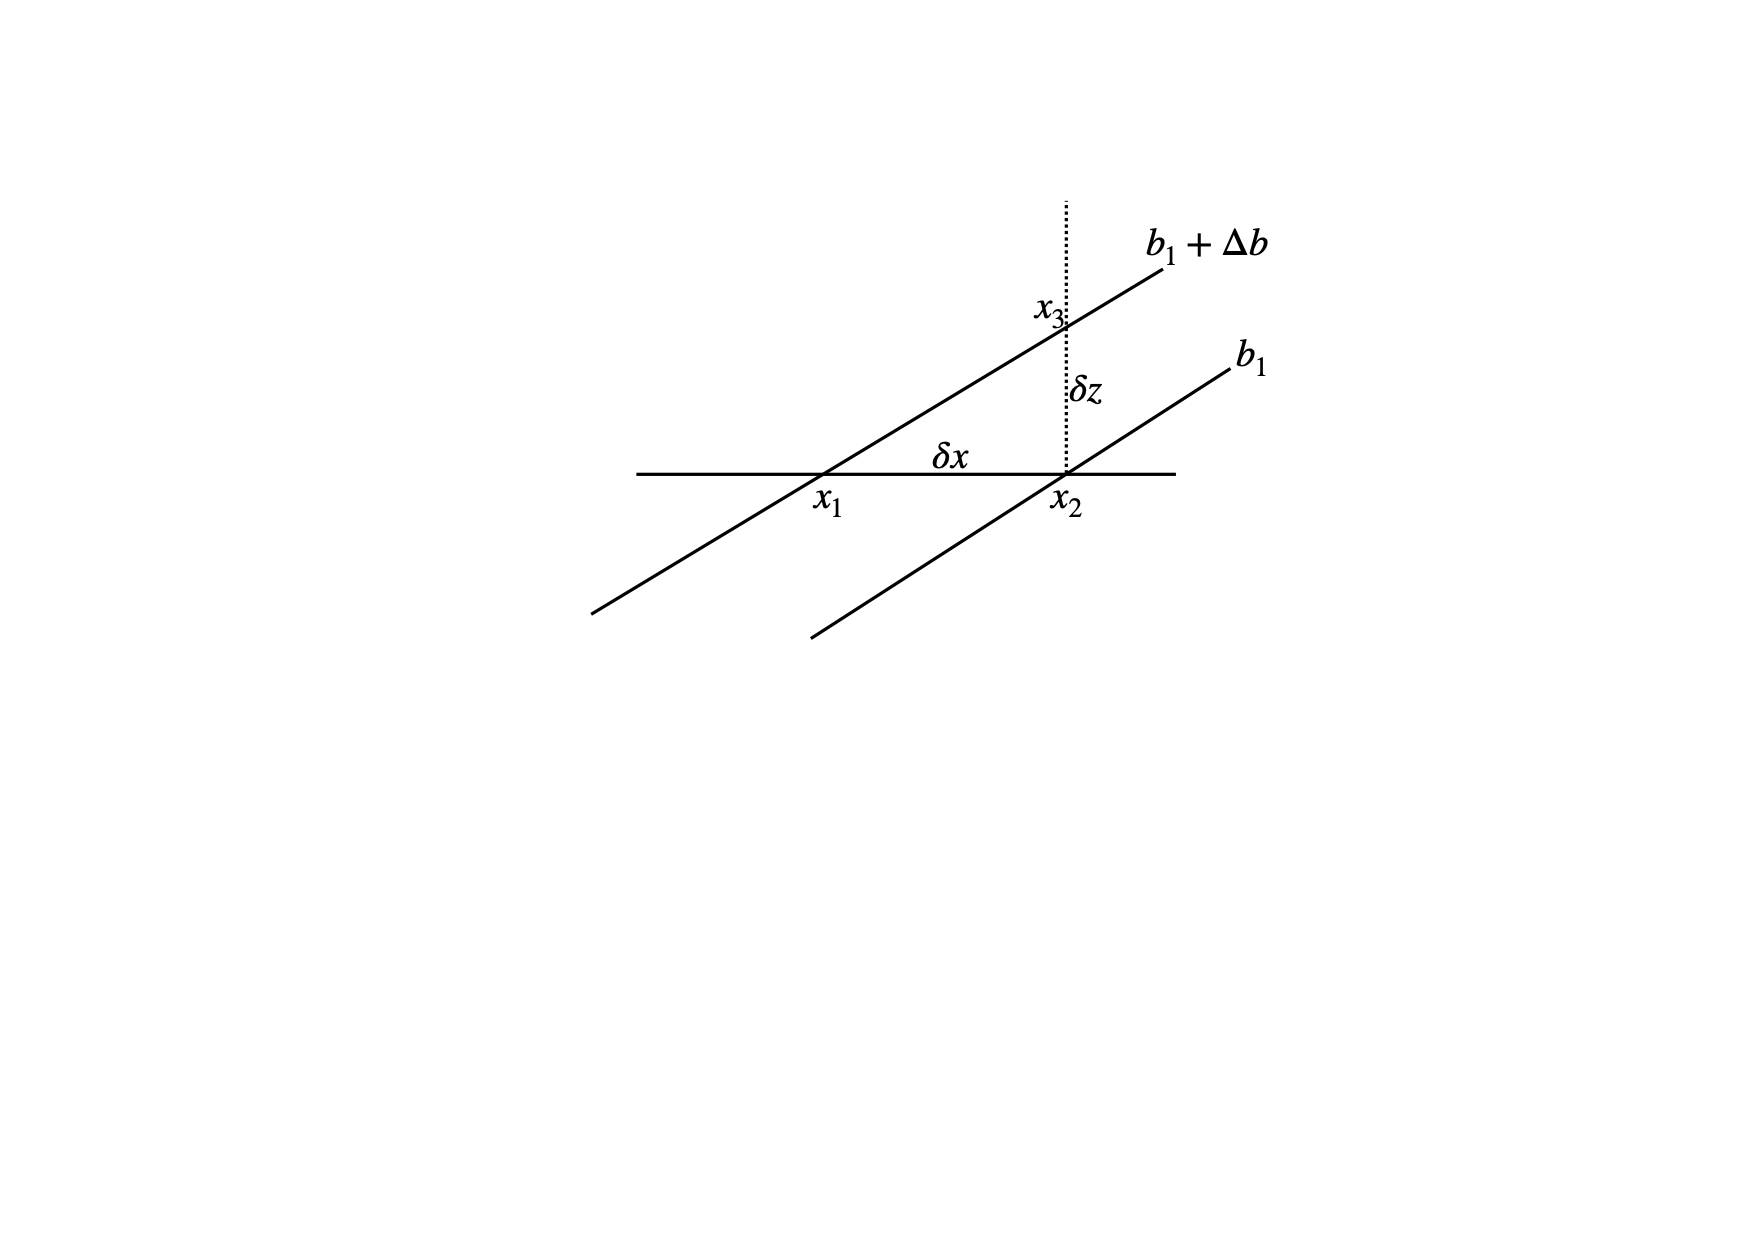
\includegraphics[width= .7 \textwidth]{figs/GD/grad.png}
\caption{Relation between gradients on isopycnal and height coordinates}
\label{fig:}
\end{figure}


can be written as

\[\begin{aligned}
A(x_2)-A(x_1) &= A(x_3)-A(x_1) - \frac{A(x_3)-A(x_2)}{\Delta b}\Delta b\\
\nabla A &= \nabla_b A + \frac{\frac{\partial A}{\partial z}}{\frac{\partial b}{\partial z}} \nabla b
\end{aligned}\]

In the QG approximation ( see Sect. \texttt{Sect:Ertel})

\[\nabla A = \nabla_b A + \frac{\frac{\partial A}{\partial z}}{N^2} \nabla \theta\]

so

\[\nabla_b Q \approx \nabla\left( f N^2 + \zeta N^2 + f_0 \frac{\partial \theta}{\partial z}\right) -\frac{\nabla\theta}{N^2}\frac{\partial }{\partial z}\left( fN^2 + \zeta N^2 + \frac{f_0}{N^2}\frac{\partial \theta}{\partial z}\right)\]

since \(f = f_0 + \beta y\) in the first term the zero order terms drops
from the gradient, whereas in the second part of the epxression the
terms \(\zeta N^2 + \frac{f_0}{N^2}\frac{\partial \theta}{\partial z}\)
are smaller by order Rossby or Richardson, so we get

\[\nabla_b Q \approx \nabla\left( \beta y N^2 + \zeta N^2 + f_0 \frac{\partial \theta}{\partial z}\right) -f_0 \frac{\nabla\theta}{N^2}\frac{\partial }{\partial z}N^2\]

reordering terms

\[\nabla_b Q \approx N^2 \nabla\left( \beta y + \zeta  + f_0 \frac{\partial }{\partial z} \frac{1}{N^2} \frac{\partial \theta}{\partial z}\right).\]

The gradient of \(Q\) on a constant density surface (isopycnal) is
approximately equal to the gradient of \(q\) on constant height
normalized by the stratification \(N^2\)

\[\nabla_b Q = N^2 \nabla q\]

and similarly

\[\frac{\partial }{\partial t}_b Q \approx N^2 \frac{\partial q}{\partial t}\]

In the case of adiabatic flow the Ertel potential vorticity is conserved
on isopycnals:

\[\frac{\partial }{\partial t}_b Q + \vec{v}\cdot\nabla_b Q = 0\]

and using the relation we have found we get

\[\frac{\partial q}{\partial t} + \vec{v}\cdot\nabla q = 0\]

the QG potential vorticity.

\subsubsection{Fluxes of potential
vorticity}\label{fluxes-of-potential-vorticity}

An important relation can be found between the meridional fluxes of
Ertel potential vorticity and the QG potential vorticity

{\[\overline{v Q}^b \approx N^2 \overline{v q}\]}

where \(\overline{( \quad  )}^b\) is the zonal average along a isopycnal
surface (constant density) and \(\overline{( \quad )}\) is the zonal
mean along a constant height surface. Let's considering a small
deviation in height of a constant density surface from the reference
level \(z_0\) to a level \(z\), then a quantity will be

\[A(z) = A(z_0) + \frac{\partial A}{\partial z}(z-z_0) + \cdots\]

but the small increments in height gives for the buoyancy increments

\[\theta = -\frac{\partial \tilde{b}}{\partial z}(z-z_0)\]

so

\[A(z) = A(z_0) - \frac{\partial A}{\partial z}\frac{1}{N^2}\theta + \cdots\]

The correction is first order in the QG expansion since

\[\frac{1}{A}\frac{\partial A}{\partial z}\frac{\theta}{N^2} \approx \frac{\theta}{N^2 H} \approx \frac{1}{Ro\,Ri}\]

so

\[\overline{A}^b = \overline{A} - \frac{1}{N^2}\overline{\frac{\partial A}{\partial z}\theta}\]

since the term on the left is on the constant buoyancy surface perturbed
from the uniform reference state and the terms on the right are on the
uniform levels. Going back to the meridional fluxes we get

{\[\overline{v Q}^b  = \overline{ f N^2 v}^b + N^2 \overline{\zeta v}^b + f_0 \overline{v\frac{\partial \theta}{\partial z}}^b\]}

the second and the third term are of the first order in QG expansion if
we substitute \(v\) with the geostrophic velocity \(v_g\), for the first
term we have

\[\overline{ f N^2 v}^b  \approx f_o N^2 \overline{v} - \frac{f_0}{N^2} \overline{\frac{\partial }{\partial z}\left(N^2 v_g\right)\theta}\]

and

\[\overline{ f N^2 v}^b  \approx f_o N^2 \overline{v} - \frac{f_0}{N^2} \frac{\partial }{\partial z}\left(N^2 \right)\overline{v_g\theta} - f_0 \overline{\frac{\partial v_g}{\partial z}\theta}\]

the last term is zero because it is the zonal mean of the geostrophic
velocity \(v_g=\frac{\partial \psi}{\partial x}\) and the term is a
total derivative in \(x\), putting together with eq \texttt{eq:vq1} we
get

{\[\overline{v Q}^b  = f_o N^2 \overline{v} + N^2 \overline{v_g\zeta_g} + N^2 f_0 \frac{\partial }{\partial z}\left(\frac{1}{N^2}\overline{v_g\theta_g}\right)\]}

because

\[q = f + \zeta_g + f_0 \frac{\partial }{\partial z} \frac{\theta}{N^2}\]

then

\[\overline{v q}  = f_o  \overline{v} +  \overline{v_g\zeta_g} + f_0 \frac{\partial }{\partial z}\left(\frac{1}{N^2}\overline{v_g\theta_g}\right)\]

and we recover eq.(\texttt{eq:qv0}).

\subsubsection{Meridional fluxes of potential
vorticity}\label{meridional-fluxes-of-potential-vorticity}

We can then compute the meridional flux of potential vorticity

\[\overline{v q} = f_0 \overline{v} +\overline{v'q'}\]

and using the results of the barotropic case

{\[\overline{v'q'} = -\frac{\partial }{\partial y} \overline{u'v'} + f_0 \frac{\partial }{\partial z} \frac{1}{N^2} \overline{v'\theta'}\]}

an important relation between the fluxes of westerly momentum and the
fluxes of two conserved quantities: the potential vorticity and the
buoyancy.
